\documentclass[conference]{IEEEtran}
\IEEEoverridecommandlockouts

\usepackage{cite}
\usepackage{amsmath,amssymb,amsfonts}
\usepackage{algorithmic}
\usepackage{graphicx}
\usepackage{textcomp}
\usepackage{xcolor}
\def\BibTeX{{\rm B\kern-.05em{\sc i\kern-.025em b}\kern-.08em
    T\kern-.1667em\lower.7ex\hbox{E}\kern-.125emX}}

\usepackage{tikz}
\usetikzlibrary{shapes.geometric, positioning}

\tikzstyle{block} = [rectangle, minimum width=2.5cm, minimum height=1cm, text centered, draw=black, font=\large]
\tikzstyle{tallblock} = [rectangle, minimum width=2.5cm, minimum height=2.5cm, text centered, draw=black, font=\large]
\tikzstyle{circleblock} = [circle, draw, minimum size=1.5cm, text centered, font=\large]
\tikzstyle{leftarrowblock} = [block, append after command={
    \pgfextra \draw[black, fill=black]
        (\tikzlastnode.west) ++(-0.4, 0) -- ++(0.4, 0.5) -- ++(0, -1) -- cycle;
    \endpgfextra
}]
\tikzstyle{tallleftarrowblock} = [tallblock, append after command={
    \pgfextra \draw[black, fill=black]
        (\tikzlastnode.west) ++(-0.4, 0) -- ++(0.4, 1.25) -- ++(0, -2.5) -- cycle;
    \endpgfextra
}]
\tikzstyle{rightarrowblock} = [block, append after command={
    \pgfextra \draw[black, fill=black]
        (\tikzlastnode.east) ++(0.4, 0) -- ++(-0.4, 0.5) -- ++(0, -1) -- cycle;
    \endpgfextra
}]


\begin{document}
\begin{sloppy}

\title{Generative AI and Empirical Software Engineering:\\A Paradigm Shift}

\author{\IEEEauthorblockN{Christoph Treude}
\IEEEauthorblockA{\textit{School of Computing and Information Systems} \\
\textit{Singapore Management University, Singapore}\\
ctreude@smu.edu.sg}
\and
\IEEEauthorblockN{Margaret-Anne Storey}
\IEEEauthorblockA{\textit{Department of Computer Science} \\
\textit{University of Victoria, Canada}\\
mstorey@uvic.ca}
}

\maketitle

\begin{abstract}
The widespread adoption of generative AI in software engineering marks a paradigm shift, offering new opportunities to design and utilize software engineering tools while influencing both developers and the artifacts they create. Traditional empirical methods in software engineering, including quantitative, qualitative, and mixed-method approaches, are well established. However, this paradigm shift introduces novel data types and redefines many concepts in the software engineering process. The roles of developers, users, agents, and researchers increasingly overlap, blurring the distinctions between these social and technical actors within the field.

This paper examines how integrating AI into software engineering challenges traditional research paradigms. It focuses on the research phenomena that we investigate, the methods and theories that we employ, the data we analyze, and the threats to validity that emerge in this new context. Through this exploration, our goal is to understand how AI adoption disrupts established software development practices that creates new opportunities for empirical software engineering research.
\end{abstract}

\begin{IEEEkeywords}
Software Engineering, Generative AI, Empirical Methods.
\end{IEEEkeywords}

\section{Introduction}

The software engineering academic and industry community is undergoing a significant transformation due to the rapid development and adoption of generative AI technologies. Many consider generative AI to be the most disruptive innovation in software engineering since the Internet~\cite{playbook}, with the potential to fundamentally change the way software is developed, evolved, and used. Others take a more conservative stance, but still acknowledge that the adoption of generative AI is driving critical and substantive changes in software development practices~\cite{notmagic}. These changes include cascading effects on delivery speed, software quality, and the developer experience.

Beyond its impact on software engineering practices, generative AI is redefining the roles of developers, users, and researchers. The boundaries between these actors are becoming increasingly blurred, opening up opportunities for novel approaches to designing, building, and studying software systems. 
Consequently, in this paper, we explore how the integration of generative AI into the software development lifecycle reshapes and challenges the empirical methods traditionally employed in software engineering research. Quantitative, qualitative, and mixed method approaches must now account for new data sources, dynamic workflows, and redefined notions of the inputs to and the outputs from the software engineering process.

It is not just the empirical methods that are disrupted, but also the nature of the research questions posed are changing. Understanding the implications of technological advances on research is a well-established area of concern in media studies and digital anthropology~\cite{digitalanthro}. For example, Marshall McLuhan~\cite{mcluhan1977laws} famously proposed four laws to analyze the impact of new technologies. Storey \emph{et al.}~\cite{playbook} describe how these laws can be applied to generative AI in software engineering:

\begin{itemize}
    \item \textbf{What does generative AI enhance or amplify?} Generative AI amplifies various software engineering tasks~\cite{hou2023large}, such as automating the writing of low-level code, which previously required significant human effort.
    \item \textbf{What does the technology make obsolete?} Traditional platforms such as Stack Overflow are seeing reduced use as generative AI provides instant coding assistance and solutions~\cite{xu2023we}, potentially reducing the reliance on community-driven resources.
    \item \textbf{What does the technology retrieve that had been obsolesced earlier?} Generative AI reintroduces the use of chat interfaces for technical assistance~\cite{shawar2007chatbots}, which were not widely utilized by developers until the advent of conversational AI models.
    \item \textbf{What does the technology reverse or flip into when pushed to extremes?} If reliance on generative AI continues to grow, foundational skills, such as learning programming from first principles, may be neglected or undervalued by new learners who overly depend on AI-generated solutions~\cite{hicks2024new}.
\end{itemize}

These laws provide a framework for understanding how generative AI disrupts traditional workflows while creating new opportunities for software engineering research. However, these disruptions also raise fundamental questions about how researchers should adapt their approaches to remain relevant and impactful. The data sources we use in our research are evolving and we must prepare for additional disruptive changes, including new phenomena, research methods, theories, and threats to validity.

This paper explores how the adoption of generative AI is reshaping empirical software engineering research. Specifically, we investigate (1) the evolving phenomena we study and the new questions that must be addressed to understand them, (2) the need for adaptation in research methods and theories to tackle the unique challenges of studying AI-driven systems, (3) the emergence of new types of data along with the opportunities and challenges they bring, and (4) the threats to validity arising from the dynamic and non-deterministic nature of AI tools.

By addressing these dimensions, this paper aims to prepare the empirical software engineering research community for a future where generative AI is not only a tool, but also an active \emph{actor}~\cite{latour2007reassembling} in software development processes. As adoption accelerates, the time to tackle these challenges is now.

\section{The Research Phenomenona We Study and the Questions We Ask}

The adoption of generative AI is fundamentally transforming the landscape of software engineering research. Mustafa Suleyman, in his book ``The Coming Wave'', describes generative AI as a ``general-purpose technology''~\cite{mustafa}, comparable to foundational innovations such as fire, the wheel, and the computer. These technologies have historically triggered ``Cambrian explosions'' of innovation, fundamentally reshaping how humans live, work, and play. Similarly, generative AI's capabilities, when combined with other disruptive technologies such as synthetic biology and augmented reality, hold the potential to drive unprecedented transformations.

Latour's actor-network theory~\cite{latour2007reassembling} emphasizes that innovation brings uncertain boundaries and fluctuating entities, making it critical for researchers to ``follow the actors'' and observe how they redefine collective existence. As generative AI becomes integrated into software engineering, traditional constructs such as ``developer'', ``source code'', and ``artifact'' are becoming more fluid, requiring empirical research to adapt to these transformations.

The roles of developers, tools, and end users are particularly affected. Developers now use AI tools to generate code, shifting their focus from writing code to designing and refining solutions. End users, empowered by AI, are increasingly taking on development tasks, further blurring the boundary between the developer and the user. Generative AI tools also actively contribute to the creation of artifacts, such as commit messages, bug reports, and UML diagrams, challenging the traditional distinction between tools and collaborators.

As discussed in the introduction, McLuhan's four laws of media~\cite{mcluhan1977laws}, as interpreted by Storey \emph{et al.}~\cite{playbook}, offer a valuable framework for analyzing these changes. The evolving definitions of ``developer'' and ``software'' further complicate these dynamics. Peter Naur's perspective~\cite{Naur} highlights that software is not merely code but theories in developers' minds about the problem being solved and how it evolves. Expanding interaction methods, such as natural language prompts, sketches~\cite{programmingbyexample}, and gestures in virtual or augmented reality environments~\cite{VRsoftware}, challenge traditional notions of ``coding'' and ``software''.

As Latour underscores, when innovations proliferate, we must be ready to observe new actors and reconsider the constructs we use to conceptualize them. For empirical software engineering researchers, this means studying emergent phenomena such as the integration of AI tools into the inner development loop and their impact on team dynamics, the evolving relationship between developers and artifacts as AI increasingly mediates their creation, and the use of synthetic data generated by AI during interactions, which redefines our understanding of developer behavior.

The implications of these transformations extend beyond technical workflows. For example, as generative AI tools learn from the traces of their interactions, they may inadvertently introduce biases or amplify existing inequities. Researchers must remain vigilant in identifying and addressing these unintended consequences.

The adoption of generative AI is not merely an enhancement of existing practices but a fundamental reshaping of the phenomena we study. By asking the right questions and adapting our conceptual frameworks, we can ensure that empirical software engineering research remains relevant and impactful in this rapidly evolving landscape.

To address these evolving phenomena and guide future research, we recommend:

\begin{itemize}
    \item Continuously refine the definitions of key constructs such as ``developer'', ``artifact'', and ``coding'' to reflect their evolving roles in AI-mediated environments.
    \item Focus on questions that explore the unique dynamics of human-AI collaboration, such as how AI tools influence creativity, collaboration, and knowledge transfer.
    \item Conduct longitudinal research to understand how AI adoption shapes software engineering practices, team dynamics, and skill development over time.
    \item Collaborate across disciplines and engage with diverse communities to uncover novel insights into the socio-technical impacts of generative AI.
\end{itemize}

\section{Research Methods and Theories}

The impact of generative AI presents challenges to the traditional methods and theories used in empirical software engineering research. Existing approaches must evolve to capture the new socio-technical dynamics introduced by AI while addressing the complexity and scale of emerging phenomena.

Empirical software engineering research has traditionally relied on a combination of quantitative, qualitative, and mixed-method approaches to analyze software-related artifacts and processes. While these methods remain foundational, generative AI introduces new challenges:

\begin{itemize}
    \item \textbf{Quantitative Methods:} The non-deterministic nature of AI output complicates traditional statistical analyses and causal inference. Researchers must account for variability in the results and the rapid evolution of AI models.
    \item \textbf{Qualitative Methods:} The blurring of socio-technical boundaries makes it difficult to isolate human behavior from AI-mediated processes. Established methods for studying developers' interactions with software systems must be adapted to include AI as an active participant. %Generative AI, however, also offers a way to accelerate the collection (via chatbots) and analysis of qualitative data.
    \item \textbf{Mixed-Method Designs:} Embedded mixed-method designs~\cite{poth} are particularly suited to study emerging phenomena. These approaches enable researchers to integrate quantitative and qualitative insights, capturing the interplay between human and AI actors in software engineering workflows. However, the AI shift introduces challenges, such as accounting for the dynamic and non-deterministic nature of AI outputs in longitudinal studies, integrating insights from AI-generated artifacts with human-generated ones, and ensuring that AI-mediated processes do not obscure critical socio-technical factors.
\end{itemize}

In addition to these challenges, all empirical studies must adapt to the dynamic nature of AI-mediated environments. Findings that are relevant at the time of the study may quickly become obsolete as AI models evolve. Longitudinal studies and iterative research designs may increasingly become a necessity.

The complexity of generative AI's impact on software engineering requires collaboration with researchers from other disciplines. Cross-disciplinary engagement can provide fresh theoretical perspectives and novel methodological approaches. For example, researchers in education can provide insight into how AI assists developers in learning and acquiring foundational programming skills, a critical factor for developer success~\cite{hicks}. Cognitive science can explore how AI influences the cognition of developers, mental models, and decision making processes, similar to how human cognition has been shaped by the Internet and social media~\cite{shallows}. Social scientists can provide valuable perspectives on how AI tools reshape team dynamics, organizational practices, and societal equity. Economists, on the other hand, can analyze data through a lens focused on higher-level patterns and systemic effects.

This interdisciplinary approach also supports the development and refinement of theoretical frameworks. For instance, theories from media studies (such as McLuhan's laws~\cite{mcluhan1977laws}), actor-network theory~\cite{latour2007reassembling}, and the Storey \emph{et al.} playbook~\cite{playbook} can be applied to examine the dynamic relationships between developers, tools, and artifacts.

Generative AI is not only a subject of study, but also a potential tool for conducting research. Recent advances demonstrate its utility in coding large volumes of qualitative data, such as mining user feedback or identifying themes in developer-AI interactions~\cite{ahmed2025can, bano2024large}, and in integrating qualitative and quantitative data, enabling mixed-method analyses that were previously challenging to conduct at scale. Generative AI may also simulate users and interactions in empirical studies, reducing the cost and time required for data collection~\cite{steinmacher}.

However, using AI as a research tool introduces its own challenges, including biases in AI-generated insights and the need for transparency in how AI is applied. Researchers must critically examine the assumptions embedded in AI systems and remain vigilant about potential ethical concerns, such as biases in training data, the opacity of AI decision-making processes, and the implications of automating tasks traditionally requiring human judgment.

As the boundaries between technical and social phenomena continue to blur, new theoretical frameworks are required to guide empirical research. Building on existing theories, researchers must consider how socio-technical systems evolve when AI becomes an active participant rather than a passive tool. In addition, they must address the implications of AI-generated synthetic data for understanding human behavior and system performance, as well as the role of AI in the reshaping of developer cognition and collaboration.

%The impact of Generative AI extends beyond traditional software engineering concerns, prompting researchers to rethink the constructs and assumptions underlying their work. Theories must accommodate the fluid roles of human and AI actors, the dynamic nature of software artifacts, and the broader societal implications of these changes.

To address these challenges, we recommend:

\begin{itemize}
    \item Developing new metrics and benchmarks to evaluate AI-mediated workflows and artifacts.
    \item Collaborating with experts in other fields to refine research methods and expand theoretical perspectives.
    \item Using AI tools to augment research processes by automating labor-intensive tasks, such as coding qualitative data, while enabling researchers to focus on higher-level interpretative and theoretical work.
    \item Establishing guidelines and guardrails to ensure transparency, address biases, and maintain critical awareness of the limitations of AI tools.
    \item Emphasizing iterative and adaptive research designs that reflect the rapid pace of technological change.
\end{itemize}

Although these strategies focus on methodologies and frameworks, another critical dimension is the data itself. As generative AI reshapes the landscape of software artifacts and interactions, understanding and leveraging these new forms of data become central to empirical research.

\section{The Data We Study}

Generative AI has transformed not only the processes and tools of software engineering but also the types of data available for empirical research. 
The important role of leveraging engineering data has been well recognized for several decades.  In the 1996 editorial for the first issue of the Empirical Software Engineering journal, Harrison and Basili defined the discipline as ``the study of software-related artifacts for the purpose of characterization, understanding, evaluation, prediction, control, management, or improvement through qualitative or quantitative analysis''~\cite{harrison1996editorial}. Almost 30 years later, this definition is fully realized. In 2022, Abou Khalil and Zacchiroli~\cite{abou2022software} conducted a meta-analysis of artifact mining in empirical software engineering, identifying over 3,000 papers that mined artifacts such as bug data, code reviews, commit metadata, forums, mail data, source code, test data, and UML diagrams. They noted common combinations of mined artifacts and purposes, including bug prediction and source code classification.

Revisiting this list of data artifacts in the generative AI era, it is evident that AI now generates many of these artifacts:

\begin{itemize}
    \item \textbf{Bug Reports}: Tools such as Buglistener automatically generate bug reports from live chats~\cite{shi2022buglistener}.
    \item \textbf{Code Review Comments}: LLaMA-Reviewer uses large language models to automate code review comments~\cite{lu2023llama}.
    \item \textbf{Commit Metadata}: The generation of automatic commit messages has proven to be valuable, with future directions highlighted~\cite{zhang2024automatic}.
    \item \textbf{Forums}: The potential of generative AI to replace platforms such as Stack Overflow is being studied for reliability~\cite{zhong2024can}.
    \item \textbf{Mail Data}: ChatGPT is used to write and reply to emails~\cite{cambiaso2023scamming}.
    \item \textbf{Source Code}: Generative AI solutions such as ChatGPT generate source code, although rigorous evaluations are essential~\cite{liu2024your}.
    \item \textbf{Test Data}: The generation of AI-powered test cases demonstrates the utility of domain knowledge~\cite{xue2024domain}.
    \item \textbf{UML Diagrams}: Large language models enable the automatic generation of image-based UML diagrams~\cite{conrardy2024image}.
\end{itemize}

These examples illustrate the diverse approaches for generating software engineering artifacts in the generative AI era. With data increasingly generated by AI, a critical question arises: What is the role of empirical software engineering researchers---are we merely to analyze AI-generated outputs?

To address this, it is essential to understand generative AI and its interactions. At the core are advanced models like GPT-4o, built using deep learning architectures and trained on diverse texts from books, articles, websites, and more. These models learn language patterns, structures, and nuances.

Interactions occur through prompts, with users providing queries or instructions. The model processes these prompts based on its training data to generate output ranging from simple text to complex artifacts such as code snippets, emails, and bug reports. The strength of Generative AI lies in producing coherent, contextually relevant responses, making it a powerful tool in software engineering.

\begin{figure}[t]
\centering
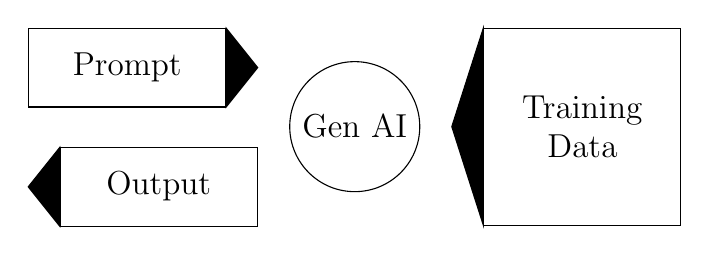
\begin{tikzpicture}
    \node (prompt) [rightarrowblock, yshift=-.5cm] at (0, 1) {Prompt};
    \node (output) [leftarrowblock, below=of prompt, yshift=.5cm, xshift=.4cm] {Output};
    \node (llm) [circleblock, right=of prompt, yshift=-0.75cm, xshift=-.2cm] {Gen AI};
    \node (data) [tallleftarrowblock, right=of llm, xshift=-.2cm] {\parbox{2cm}{\centering Training \ Data}};
\end{tikzpicture}
\caption{New types of data amenable to empirical software engineering research in the era of generative AI adoption: training data, prompts, and output.}
\label{fig}
\end{figure}

The widespread adoption of generative AI tools presents new opportunities for empirical research on emerging data types. Figure~\ref{fig} highlights these opportunities: analyzing training data, examining prompts and interactions, and studying outputs. Each area provides rich insights to help understand and advance software engineering practices in the era of generative AI.

As empirical software engineering researchers, we are well placed to analyze the training data underpinning generative AI. Software-related data is inherently complex, involving diverse types, quality levels, and extensive interconnections relevant to software engineering tasks. For example, training data quality heavily influences AI model performance. As an example, Lin \emph{et al.}~\cite{lin2024improving} demonstrate that experience-aware oversampling can improve the correctness, informativeness, and relevance of reviews generated by a model without adding new data, underscoring the importance of high quality input. Similarly, adding contextual details to training data also improves model capabilities. For instance, Nguyen \emph{et al.}~\cite{nguyen2024encoding} found that incorporating the version history significantly improved the detection of code clones, showing that expanding the scope of training data can improve AI performance. At the same time, addressing biases in training data is critical to ensuring fairness. For example, Treude and Hata~\cite{treude2023she} revealed gender biases in models trained on software data, while Sami \emph{et al.}~\cite{sami2023case} found similar biases in DALL-E-2 outputs. These findings highlight the need for interventions during training to ensure equitable AI outcomes.

Beyond training data, the study of prompts and interactions offers rich avenues for exploration. The rise of generative AI requires us to extend existing research traditions on developer interactions with artifacts such as bug reports~\cite{davies2014s}, commits~\cite{alali2008s}, and code reviews~\cite{li2017they} to encompass developer-AI interactions. For instance, the DevGPT dataset~\cite{xiao2024devgpt}, containing nearly 5,000 developer-ChatGPT conversations, offers insights into prompt usage, conversation structures, and modifications to AI-generated code. As the adoption of generative AI grows, expanding data sources beyond shared conversations to include observational studies and surveys will be essential to fully understand these interactions.

Finally, the quality and implications of the AI generative output are central to ongoing research. Although studies like those by Liu \emph{et al.}~\cite{liu2024no} and Yetistiren \emph{et al.}~\cite{yetistiren2022assessing} focus on the accuracy of AI-generated artifacts, a broader perspective is needed. Inspired by McLuhan’s laws and Storey \emph{et al.}~\cite{playbook}, it is important to assess what might be lost as generative AI replaces traditional resources. For example, Stack Overflow brought significant benefits, but also led to reduced documentation comprehensiveness~\cite{parnin2012crowd}. Similarly, as AI-generated artifacts replace human-driven content, we risk losing depth, diversity, and community engagement.

To explore these specific areas, we recommend:

\begin{itemize}
    \item Investigating the nuances in human coding practices that may be lost when relying on AI-generated code.
    \item Analyzing the insights that are overlooked in AI-automated bug identification processes.
    \item Examining how mentorship dynamics are altered in AI-driven code reviews and how these changes impact developer growth.
    \item Assessing the depth and informativeness of AI-generated commit documentation compared to human-generated equivalents.
    \item Evaluating the limitations of AI-generated test oracles in capturing human intuition.
    \item Studying the effects of generative AI on community engagement, particularly in contexts where it replaces collaborative platforms like Stack Overflow.
\end{itemize}

By looking beyond output quality and critically assessing the broader impacts of generative AI, researchers can help avoid eroding valuable aspects of software engineering culture and practice.

\section{Reconsidering Threats to Validity}

The adoption of generative AI in software engineering introduces new threats to validity that challenge established practices in empirical research. These threats stem from the dynamic, non-deterministic nature of AI systems, the evolving constructs we study, and the reliance on AI-generated data and tools in research processes.

Construct validity refers to the extent to which a study measures what it claims to measure. Generative AI disrupts traditional constructs in software engineering research. Concepts such as ``developer'', ``source code'', and ``artifact'' are evolving as AI tools take on active roles in software development. For instance, when natural language prompts replace programming languages, the definition of ``coding'' becomes ambiguous. As AI tools blur the boundaries between social and technical phenomena, traditional constructs may no longer capture the full complexity of the systems being studied. McLuhan's tetrad~\cite{mcluhan1977laws} provides a framework for understanding how these constructs evolve by analyzing what AI enhances, obsolesces, retrieves, and reverses.

Internal validity refers to the degree to which a study can establish causal relationships. Generative AI complicates this process in several ways. The inherent variability in AI-generated output makes it difficult to replicate studies and establish causality. For example, the same prompt can yield different results across executions, even within the same model. Frequent updates to generative AI models further complicate longitudinal analyses, as studies conducted on older versions may lose relevance as the models evolve and their behavior changes.

External validity refers to the generalizability of the study findings. The unique characteristics of generative AI introduce new challenges in this regard. Studies focusing on proprietary or closed-source models (e.g., OpenAI's GPT) may produce findings that are not applicable to other models or contexts. Similarly, research conducted in controlled settings may not capture the complexities of real-world scenarios, where AI tools interact with a diverse range of users and systems. The rapid adoption of generative AI underscores the need for studies that reflect the dynamic environments in which these tools are applied.

Generative AI models are trained on large datasets that reflect societal biases, which can distort empirical findings. Research has shown that generative AI can perpetuate gender and cultural biases~\cite{treude2023she, sami2023case}. For example, AI-generated code reviews or documentation may inadvertently include biased language or assumptions. The use of biased AI-generated data in research raises ethical concerns, particularly when such data informs decision-making or trains future AI systems.

The use of generative AI in empirical research introduces additional threats. When AI is used to code qualitative data or simulate users, the biases inherent in the underlying models can influence the findings. Furthermore, many AI tools function as ``black boxes'', making it difficult to discern how their output was generated. This lack of transparency complicates the interpretation of the results and hinders the reproducibility of the studies. Researchers who rely heavily on AI tools may inadvertently overlook critical nuances or context that would have been evident in manual analyses.

To address these threats, researchers must adopt strategies that ensure rigor and reliability:

\begin{itemize}
    \item Whenever possible, researchers should prioritize open source models to enable greater transparency and control, reduce dependence on proprietary tools, and improve replicability.
    \item Iterative and adaptive research designs can accommodate the rapid evolution of AI models and the dynamic nature of AI-generated outputs.
    \item Researchers should regularly review and refine their constructs to ensure that they remain relevant in the context of evolving phenomena.
    \item Mixed methods~\cite{poth, mixedthreats} are particularly well suited to address the complex and emergent nature of AI-mediated phenomena and should be applied with care.
    \item Researchers should critically evaluate assumptions and biases embedded in AI tools and transparently report their limitations.
\end{itemize}

By proactively addressing these threats, empirical software engineering researchers can maintain the validity and reliability of their findings in the era of generative AI.

\section{Final Thoughts}

Generative AI is fundamentally reshaping empirical software engineering research, presenting both opportunities and challenges. Its integration into the software development lifecycle is not simply enhancing existing practices but driving radical transformations that require researchers to rethink their approaches to data, methods, and theoretical frameworks.

This paper has outlined how empirical software engineering must evolve to address these changes. Researchers must reassess the phenomena they study, redefining constructs such as ``developer'' and ``artifact'' in light of active participation of AI. Research methods must adapt to the dynamic nature of AI-mediated workflows, incorporating interdisciplinary perspectives, and utilizing mixed-method designs. New data sources, including AI-generated artifacts and synthetic datasets, should be embraced, but with attention to challenges such as bias and interpretability. In addition, adaptive study designs, open source tools, and critical assessments of AI limitations are essential to mitigate novel threats to validity.

The adoption of generative AI is accelerating, and its impact on software engineering research is likely to expand in complexity and scope. Although its immediate benefits, such as increased productivity and automation, are clear, the broader implications for the field demand careful consideration. Overreliance on AI could undermine foundational skills, and biases in AI-generated data risk perpetuating inequities.

Thus, we hope this paper sparks discussion and collective action within the research community to address these challenges and seize the opportunities generative AI presents. Thoughtfully navigating this transformative era will determine whether generative AI becomes a tool for meaningful innovation or a source of unintended consequences. By combining rigorous empirical research with a forward-looking perspective, the software engineering community can lead the way in this exciting, yet challenging new era.

% Generated by IEEEtran.bst, version: 1.14 (2015/08/26)
\begin{thebibliography}{10}
\providecommand{\url}[1]{#1}
\csname url@samestyle\endcsname
\providecommand{\newblock}{\relax}
\providecommand{\bibinfo}[2]{#2}
\providecommand{\BIBentrySTDinterwordspacing}{\spaceskip=0pt\relax}
\providecommand{\BIBentryALTinterwordstretchfactor}{4}
\providecommand{\BIBentryALTinterwordspacing}{\spaceskip=\fontdimen2\font plus
\BIBentryALTinterwordstretchfactor\fontdimen3\font minus \fontdimen4\font\relax}
\providecommand{\BIBforeignlanguage}[2]{{%
\expandafter\ifx\csname l@#1\endcsname\relax
\typeout{** WARNING: IEEEtran.bst: No hyphenation pattern has been}%
\typeout{** loaded for the language `#1'. Using the pattern for}%
\typeout{** the default language instead.}%
\else
\language=\csname l@#1\endcsname
\fi
#2}}
\providecommand{\BIBdecl}{\relax}
\BIBdecl

\bibitem{playbook}
M.-A. Storey, D.~Russo, N.~Novielli, T.~Kobayashi, and D.~Wang, ``A disruptive research playbook for studying disruptive innovations,'' \emph{ACM Transactions on Software Engineering and Methodology}, vol.~33, no.~8, pp. 1--29, 2024.

\bibitem{notmagic}
T.~Leaver and S.~Srdarov, ``{ChatGPT} isn't magic: The hype and hypocrisy of generative artificial intelligence ({AI}) rhetoric,'' \emph{M/C Journal}, vol.~26, 10 2023.

\bibitem{digitalanthro}
H.~A. Horst and D.~Miller, \emph{Digital anthropology}.\hskip 1em plus 0.5em minus 0.4em\relax Routledge, 2020.

\bibitem{mcluhan1977laws}
M.~McLuhan, ``Laws of the media,'' \emph{ETC: A Review of General Semantics}, pp. 173--179, 1977.

\bibitem{hou2023large}
X.~Hou, Y.~Zhao, Y.~Liu, Z.~Yang, K.~Wang, L.~Li, X.~Luo, D.~Lo, J.~Grundy, and H.~Wang, ``Large language models for software engineering: A systematic literature review,'' \emph{ACM Transactions on Software Engineering and Methodology}, 2023.

\bibitem{xu2023we}
B.~Xu, T.-D. Nguyen, T.~Le-Cong, T.~Hoang, J.~Liu, K.~Kim, C.~Gong, C.~Niu, C.~Wang, B.~Le \emph{et~al.}, ``Are we ready to embrace generative {AI} for software {Q\&A}?'' in \emph{Proceedings of the IEEE/ACM International Conference on Automated Software Engineering}.\hskip 1em plus 0.5em minus 0.4em\relax IEEE, 2023, pp. 1713--1717.

\bibitem{shawar2007chatbots}
B.~A. Shawar and E.~Atwell, ``Chatbots: Are they really useful?'' \emph{Journal for Language Technology and Computational Linguistics}, vol.~22, no.~1, pp. 29--49, 2007.

\bibitem{hicks2024new}
C.~M. Hicks, C.~Lee, and K.~Foster-Marks, ``The new developer: {AI} skill threat, identity change \& developer thriving in the transition to {AI}-assisted software development,'' 2024.

\bibitem{latour2007reassembling}
B.~Latour, \emph{Reassembling the social: An introduction to actor-network-theory}.\hskip 1em plus 0.5em minus 0.4em\relax Oup Oxford, 2007.

\bibitem{mustafa}
M.~Suleyman, \emph{\BIBforeignlanguage{en}{The coming wave}}.\hskip 1em plus 0.5em minus 0.4em\relax New York, NY: Crown Publishing Group, Sep. 2023.

\bibitem{Naur}
P.~Naur, ``Programming as theory building,'' \emph{Microprocessing and Microprogramming}, vol.~15, no.~5, pp. 253--261, 1985.

\bibitem{programmingbyexample}
D.~C. Halbert, \emph{Programming by example}.\hskip 1em plus 0.5em minus 0.4em\relax University of California, Berkeley, 1984.

\bibitem{VRsoftware}
J.~M. Gonzalez-Barahona, ``{IDEs} in the age of {LLMs} and {XR},'' in \emph{Proceedings of the ACM/IEEE Workshop on Integrated Development Environments}, 2024, pp. 66--69.

\bibitem{poth}
C.~N. Poth, \emph{Innovation in mixed methods research: A practical guide to integrative thinking with complexity}.\hskip 1em plus 0.5em minus 0.4em\relax Los Angeles: SAGE, 2018.

\bibitem{hicks}
C.~M. Hicks, C.~S. Lee, and M.~Ramsey, ``Developer thriving: Four sociocognitive factors that create resilient productivity on software teams,'' \emph{IEEE Software}, vol.~41, no.~4, pp. 68--77, 2024.

\bibitem{shallows}
N.~Carr, \emph{The shallows: What the {Internet} is doing to our brains}.\hskip 1em plus 0.5em minus 0.4em\relax WW Norton \& Company, 2020.

\bibitem{ahmed2025can}
T.~Ahmed, P.~Devanbu, C.~Treude, and M.~Pradel, ``Can {LLMs} replace manual annotation of software engineering artifacts?'' in \emph{Proceedings of the International Conference on Mining Software Repositories}, 2025.

\bibitem{bano2024large}
M.~Bano, R.~Hoda, D.~Zowghi, and C.~Treude, ``Large language models for qualitative research in software engineering: Exploring opportunities and challenges,'' \emph{Automated Software Engineering}, vol.~31, no.~1, p.~8, 2024.

\bibitem{steinmacher}
M.~Gerosa, B.~Trinkenreich, I.~Steinmacher, and A.~Sarma, ``Can {AI} serve as a substitute for human subjects in software engineering research?'' \emph{Automated Software Engineering}, vol.~31, no.~1, p.~13, 2024.

\bibitem{harrison1996editorial}
\BIBentryALTinterwordspacing
W.~Harrison and V.~R. Basili, ``Editorial,'' \emph{Empirical Software Engineering}, vol.~1, no.~1, p. 5–10, 1996. [Online]. Available: \url{http://dx.doi.org/10.1007/BF00125808}
\BIBentrySTDinterwordspacing

\bibitem{abou2022software}
Z.~Abou~Khalil and S.~Zacchiroli, ``Software artifact mining in software engineering conferences: A meta-analysis,'' in \emph{Proceedings of the ACM/IEEE International Symposium on Empirical Software Engineering and Measurement}, 2022, pp. 227--237.

\bibitem{shi2022buglistener}
L.~Shi, F.~Mu, Y.~Zhang, Y.~Yang, J.~Chen, X.~Chen, H.~Jiang, Z.~Jiang, and Q.~Wang, ``Buglistener: identifying and synthesizing bug reports from collaborative live chats,'' in \emph{Proceedings of the International Conference on Software Engineering}, 2022, pp. 299--311.

\bibitem{lu2023llama}
J.~Lu, L.~Yu, X.~Li, L.~Yang, and C.~Zuo, ``{LLaMA-Reviewer}: Advancing code review automation with large language models through parameter-efficient fine-tuning,'' in \emph{Proceedings of the IEEE International Symposium on Software Reliability Engineering}.\hskip 1em plus 0.5em minus 0.4em\relax IEEE, 2023, pp. 647--658.

\bibitem{zhang2024automatic}
Y.~Zhang, Z.~Qiu, K.-J. Stol, W.~Zhu, J.~Zhu, Y.~Tian, and H.~Liu, ``Automatic commit message generation: A critical review and directions for future work,'' \emph{IEEE Transactions on Software Engineering}, 2024.

\bibitem{zhong2024can}
L.~Zhong and Z.~Wang, ``Can {LLM} replace {Stack Overflow}? {A} study on robustness and reliability of large language model code generation,'' in \emph{Proceedings of the AAAI Conference on Artificial Intelligence}, vol.~38, no.~19, 2024, pp. 21\,841--21\,849.

\bibitem{cambiaso2023scamming}
E.~Cambiaso and L.~Caviglione, ``Scamming the scammers: Using {ChatGPT} to reply mails for wasting time and resources,'' \emph{arXiv preprint arXiv:2303.13521}, 2023.

\bibitem{liu2024your}
J.~Liu, C.~S. Xia, Y.~Wang, and L.~Zhang, ``Is your code generated by {ChatGPT} really correct? {Rigorous} evaluation of large language models for code generation,'' \emph{Advances in Neural Information Processing Systems}, vol.~36, 2024.

\bibitem{xue2024domain}
Z.~Xue, L.~Li, S.~Tian, X.~Chen, P.~Li, L.~Chen, T.~Jiang, and M.~Zhang, ``Domain knowledge is all you need: A field deployment of {LLM}-powered test case generation in {FinTech} domain,'' in \emph{Proceedings of the IEEE/ACM International Conference on Software Engineering: Companion Proceedings}, 2024, pp. 314--315.

\bibitem{conrardy2024image}
A.~Conrardy and J.~Cabot, ``From image to {UML}: First results of image based {UML} diagram generation using {LLMs},'' \emph{arXiv preprint arXiv:2404.11376}, 2024.

\bibitem{lin2024improving}
H.~Y. Lin, P.~Thongtanunam, C.~Treude, and W.~Charoenwet, ``Improving automated code reviews: Learning from experience,'' in \emph{Proceedings of the International Conference on Mining Software Repositories}, 2024, pp. 278--283.

\bibitem{nguyen2024encoding}
H.~Nguyen, P.~Thongtanunam, and C.~Treude, ``Encoding version history context for better code representation,'' in \emph{Proceedings of the International Conference on Mining Software Repositories}, 2024, pp. 631--636.

\bibitem{treude2023she}
C.~Treude and H.~Hata, ``She elicits requirements and he tests: Software engineering gender bias in large language models,'' in \emph{Proceedings of the International Conference on Mining Software Repositories}.\hskip 1em plus 0.5em minus 0.4em\relax IEEE, 2023, pp. 624--629.

\bibitem{sami2023case}
M.~Sami, A.~Sami, and P.~Barclay, ``A case study of fairness in generated images of large language models for software engineering tasks,'' in \emph{Proceedings of the IEEE International Conference on Software Maintenance and Evolution}.\hskip 1em plus 0.5em minus 0.4em\relax IEEE, 2023, pp. 391--396.

\bibitem{davies2014s}
S.~Davies and M.~Roper, ``What's in a bug report?'' in \emph{Proceedings of the ACM/IEEE International Symposium on Empirical Software Engineering and Measurement}, 2014, pp. 1--10.

\bibitem{alali2008s}
A.~Alali, H.~Kagdi, and J.~I. Maletic, ``What's a typical commit? {A} characterization of open source software repositories,'' in \emph{Proceedings of the IEEE International Conference on Program Comprehension}.\hskip 1em plus 0.5em minus 0.4em\relax IEEE, 2008, pp. 182--191.

\bibitem{li2017they}
Z.-X. Li, Y.~Yu, G.~Yin, T.~Wang, and H.-M. Wang, ``What are they talking about? {Analyzing} code reviews in pull-based development model,'' \emph{Journal of Computer Science and Technology}, vol.~32, pp. 1060--1075, 2017.

\bibitem{xiao2024devgpt}
T.~Xiao, C.~Treude, H.~Hata, and K.~Matsumoto, ``{DevGPT}: Studying developer-{ChatGPT} conversations,'' in \emph{Proceedings of the International Conference on Mining Software Repositories}, 2024, pp. 227--230.

\bibitem{liu2024no}
Z.~Liu, Y.~Tang, X.~Luo, Y.~Zhou, and L.~F. Zhang, ``No need to lift a finger anymore? {Assessing} the quality of code generation by {ChatGPT},'' \emph{IEEE Transactions on Software Engineering}, 2024.

\bibitem{yetistiren2022assessing}
B.~Yetistiren, I.~Ozsoy, and E.~Tuzun, ``Assessing the quality of {GitHub} {Copilot’s} code generation,'' in \emph{Proceedings of the International Conference on Predictive Models and Data Analytics in Software Engineering}, 2022, pp. 62--71.

\bibitem{parnin2012crowd}
C.~Parnin, C.~Treude, L.~Grammel, and M.-A. Storey, ``Crowd documentation: Exploring the coverage and the dynamics of {API} discussions on {Stack Overflow},'' \emph{Georgia Institute of Technology, Tech. Rep}, vol.~11, 2012.

\bibitem{mixedthreats}
X.~Yu and D.~Khazanchi, ``Using embedded mixed methods in studying is phenomena: Risks and practical remedies with an illustration,'' \emph{Using Embedded Mixed Methods in Studying IS Phenomena: Risks and Practical Remedies with an Illustration}, vol.~41, 2017.

\end{thebibliography}


\end{sloppy}
\end{document}